\documentclass[11pt]{article}

% ---------------------------------------------------------------------------
% Masculine social formations in long nineteenth-century fiction (STM, K=7)
% Draft for Humanities and Social Sciences Communications (also suitable, with
% minor adjustment, for Digital Scholarship in the Humanities).
% HSSC requires the Methods section to appear in the body (not at the end);
% this draft keeps a conventional IMRaD-with-Methods-in-body structure that
% also satisfies DSH.
% Figures are read from the verified output package:
%   outputs/hssc_figures_full_1930_k7_seven_concepts/
% Numbers in text/tables are taken from the STM run, not from memory.
% References reuse only the author's vetted set (references.bib); none were
% invented, and bibliographic details were verified against publisher records.
% Floats use [htbp] and are placed at first mention so they distribute through
% the text rather than collecting at the end.
% ---------------------------------------------------------------------------

\usepackage[utf8]{inputenc}
\usepackage[T1]{fontenc}
\usepackage[margin=1in]{geometry}
\usepackage{graphicx}
\usepackage{booktabs}
\usepackage{array}
\usepackage{caption}
\usepackage{amsmath}
\usepackage[numbers,sort&compress]{natbib}
\usepackage[hidelinks]{hyperref}

\graphicspath{{../figures/}}

\title{\textbf{From Gentlemanly Status to Professional Breadwinner:\\
Structural Topic Modeling of Masculine Formations in\\
English-Language Fiction, 1771--1930}}
\author{[Author(s) redacted for review]}
\date{}

\begin{document}
\maketitle

\begin{abstract}
\noindent Gender theory holds that masculinity is plural and historically
dynamic, yet measuring that plurality across a literary corpus invites two
methodological hazards: fixing the number of topics so that it reproduces one's
own categories (circularity), and reading false precision from textual segments
that are not independent. We confront both in a structural topic model (STM) of
150 English-language (British and American) novels (1771--1930), divided into
9{,}271 segments and modeled with period and author-gender metadata. Seven
theory-driven masculine families serve as an interpretive lens rather than a
target: model size is fixed on a substantive criterion---the smallest number of
topics at which a professional-commercial formation becomes distinct
($K=7$)---and uncertainty is estimated by bootstrapping whole novels rather than
segments. Six of the seven families separate as distinct topics; the seventh,
Christian moralism, does not separate until $K=9$, dispersed across domestic and
historical-religious discourse. Bootstrapped between-period differences are
statistically robust for every formation: professional-commercial masculinity
rises and a sentimental register declines most strongly, while the
much-discussed ``decline of the gentleman,'' though robust, is roughly five
times smaller in magnitude---so the shift is better described as a large new
formation emerging \emph{alongside} a modest erosion of the old than as a
symmetric replacement. These trajectories converge with established literary
historiography, corroborating the formations without proving them. We conclude
that topic modeling can
evidence the \emph{existence} and \emph{historical reweighting} of plural
masculinities, but cannot certify their \emph{number}---which remains a question
for theory and interpretation rather than for the model.
\end{abstract}

\noindent\textbf{Keywords:} computational literary studies; digital humanities;
structural topic modeling; masculinity; nineteenth-century fiction; gender
history; distant reading; uncertainty quantification

\section{Introduction}

That masculinity is plural is now a settled premise of gender studies. Since
\citet{connell1995masculinities}, scholars have treated manhood not as a single
essence but as a field of competing arrangements---hegemonic and marginal,
residual and emergent---organized through class, work, domesticity, religion,
and empire. For the long nineteenth century, historians and literary critics
have shown in detail how a gentleman, a father, a soldier, a clerk, and a man of
God inhabit different and often incompatible scripts of manliness
\citep{tosh1999mans,davidoff1987family,sussman1995victorian,adams1995dandies,mallett2015victorian}.
What this scholarship establishes through close reading, however, it rarely
measures at scale: how the \emph{relative weight} of these scripts shifts across
a century of fiction, and whether such shifts can be observed reproducibly
rather than inferred from a handful of canonical examples.

Computational literary studies promises exactly this kind of aggregate evidence
\citep{moretti2000conjectures,jockers2013macroanalysis,underwood2019distant,piper2018enumerations,heuser2012quantitative}.
Topic modeling, in particular, infers recurrent thematic structure without
predefining every category, and structural topic modeling (STM) lets
document metadata such as period and authorship inform that structure
\citep{roberts2019stm}. But applying these tools to a theoretical construct like
plural masculinity raises two hazards that are easy to overlook. The first is
\emph{circularity}: if one fixes the number of topics so that it reproduces a
pre-chosen number of categories, the finding that ``the model recovers the
categories'' is guaranteed by construction. The second is \emph{false
precision}: novels are typically split into many segments to capture local
variation, but segments from the same book are not independent, so significance
tests that treat them as such report implausibly tiny $p$-values. Both hazards
push toward confident conclusions that the data do not support.

This article treats those two hazards as its central methodological problem
rather than as footnotes. We model masculinity not as a list of male-coded words
but as a set of recurrent thematic \emph{formations}---constellations of
co-occurring vocabulary through which masculine roles become socially legible.
Seven theory-driven families (gentlemanly status, domestic paternalism,
aristocratic chivalry, professional breadwinning, imperial adventure, Christian
moralism, and sentimental manhood) serve as an interpretive lens, not as a target
to be matched. Three design choices follow from this stance: we fix the model
size on a substantive criterion independent of the taxonomy, estimate uncertainty
by resampling whole novels, and validate the resulting formations against
independent literary historiography. A topic model never ``discovers''
masculinity in the sense in which a critic interprets a scene; it produces
artifacts that become evidence only when read cautiously
\citep{buurma2015fictionality}.

The analysis yields three findings. First, six of the seven theoretical
formations separate as distinct topics, and their \emph{differential}
separability is itself informative: Christian moralism does not emerge as its own
topic until a higher model size, because in this corpus religious manliness is
expressed \emph{through} domestic discourse rather than apart from it. Second,
the corpus exhibits a robust rise of a professional-commercial formation and a
robust decline of a sentimental register; the celebrated ``decline of the
gentleman,'' though also statistically robust, is roughly five times smaller in
magnitude than the breadwinner's rise---a mild corrective to a strand of the
qualitative literature that treats the two movements as a symmetric exchange.
Third, and most generally, topic modeling
can support claims about the existence and historical reweighting of plural
masculine formations while remaining unable to certify how many such formations
exist, because the number of topics is a modeling choice rather than a quantity
the data determine.

\section{Background}

Topic modeling entered literary history as a way to infer themes without
hand-coding them, whether to mine the ``great unread'' for passages of interest
\citep{tangherlini2013trawling} or to chart themes at corpus scale.
\citet{jockers2013significant}, the closest precedent to this
study, used topics as proxies for literary themes and related their prevalence to
author gender, nationality, and date. We depart from that work in two respects:
we adopt STM rather than latent Dirichlet allocation \citep{blei2003lda} so that
period and authorship inform topical prevalence directly
\citep{roberts2014structural,roberts2019stm}, and we narrow the focus to the
historical movement of masculine formations specifically. A complementary strand
models gender directly rather than thematically: \citet{underwood2018transformation}
show that the linguistic marking of gendered characters weakens across
English-language fiction since the nineteenth century even as the share of
fiction written by women declines. We instead track masculine \emph{thematic}
formations and their changing prevalence, a different and narrower object. The
interpretive stakes of the method are themselves contested. \citet{buurma2015fictionality} reads topic
models as fictions that can usefully \emph{denaturalize} familiar texts, and
\citet{goldstone2014quiet} show that topics can surface gradual transformations
invisible to explicit debate. Both caution against treating model output as a
conclusion. So do the technical diagnostics: \citet{chang2009reading} demonstrate
that better-fitting models can be \emph{less} interpretable, and
\citet{mimno2011optimizing} formalize semantic coherence as a guard against
topics that are statistically fitted but humanly meaningless. More recent work
sharpens both cautions: \citet{hoyle2021automated} show that automated coherence
metrics can crown models that human readers reject, and \citet{da2019computational}
argues that many computational literary findings are statistically fragile or
non-reproducible. We take these as reasons to keep human interpretation in the
loop and---as Section~\ref{sec:modelsel} makes explicit---to refuse coherence as
the sole arbiter of model size, rather than as grounds to abandon the method.

On the substantive side, the scholarship of masculinity supplies both the
formations we look for and the historiography against which we test them.
\citet{connell1995masculinities} makes plurality analytically primary and warns
against reducing masculinity to a single dictionary. \citet{davidoff1987family}
and \citet{tosh1999mans} trace how middle-class manhood was produced through
family, business, and religion, with domesticity a central but contradictory
ideal. \citet{sussman1995victorian}, \citet{adams1995dandies},
\citet{solinger2012becoming}, and \citet{mallett2015victorian} track masculine
styles across gentility, asceticism, muscular Christianity, aestheticism, and
self-fashioning. This body of work both motivates a broad operational vocabulary
and provides the external benchmark---an expected chronology of domestic,
adventurous, and commercial manhood---against which a model's trajectories can be
judged.

\section{Data and methods}

\subsection{Corpus and segmentation}
The corpus is the English-language subset of Andrew Piper's txtLAB Novel450
dataset \citep{piper2016txtlab}: 150 British and American novels published
between 1771 and 1930. Each novel is
divided into non-overlapping, sentence-aware windows of approximately 2{,}000
words, yielding 9{,}271 segments and 6{,}562{,}588 retained tokens (mean
$\approx 708$ tokens per segment after preprocessing). Segmentation makes the
model sensitive to local thematic variation---a single novel may contain
domestic, commercial, and adventurous passages---while non-overlapping windows
limit dependence between adjacent units. Because segments from the same novel
nevertheless remain correlated, all prevalence estimates are aggregated to the
novel level before comparison (Section~\ref{sec:inference}). The 150 novels span
five periods---Georgian (41), Early Victorian (40), Late Victorian (36),
Edwardian (18), and Early Modernist (15)---and two author-gender categories (81
male, 69 female).

\subsection{Preprocessing}
Preprocessing is deliberately conservative: tokens are lowercased and normalized,
common stopwords and dialogue contractions removed, conservative plural
normalization applied, and very rare or ubiquitous terms excluded (retained in at
least 25 and at most 65\% of documents). A document-specificity filter removes
2{,}604 terms concentrated in individual novels, reducing the chance that
protagonist names or single-work vocabulary become spurious topics; the final
vocabulary holds 15{,}946 terms. Masculinity-relevant common words (e.g.\
\emph{sir}, \emph{gentleman}, \emph{father}, \emph{master}, \emph{man},
\emph{men}, \emph{work}, \emph{money}) are protected from removal. To verify that
this protection does not drive the results, we re-ran the entire pipeline at
$K=7$ with no protected terms, so that all vocabulary was subject to the same
frequency and document-specificity filters. The vocabulary changed by a single
term ($15{,}945$ vs.\ $15{,}946$), the same six formations emerged, and every
period trajectory was unchanged within rounding (for example, professional
breadwinning $0.02\rightarrow0.39$ vs.\ $0.02\rightarrow0.37$; sentimental
manhood $0.35\rightarrow0.02$ in both). The protected list is therefore a
convenience for interpretation, not a determinant of the findings; more
generally, because the masculine families are applied only after estimation
(Section~4.3), they shape labels rather than the topics, prevalences, or
trajectories the model produces.

\subsection{Model and theory-guided labeling}
Models are estimated with the \texttt{stm} package \citep{roberts2019stm} using
Spectral initialization and the prevalence formula \texttt{period +
author\_gender}. Interpretation is guided by the seven masculine families
introduced above, derived a priori from the scholarship in Section~2. A topic is
flagged as a candidate for a family when at least two of its highest-probability
or FREX (frequency--exclusivity) words fall in that family's vocabulary; final
labels reflect a reading of probability words, FREX words, and representative
segments. Crucially, the families are an interpretive lens applied \emph{after}
estimation; they never enter model fitting or the choice of model size.

\subsection{Choosing the number of topics}
\label{sec:modelsel}
We compared models from $K=3$ to $K=15$ on held-out likelihood, residuals,
semantic coherence, and exclusivity (Table~\ref{tab:modelcomp},
Fig.~\ref{fig:modelcomp}). Three diagnostics---held-out likelihood, residuals,
and exclusivity---improve monotonically with $K$, as they generally do; semantic
coherence is highest at low $K$ ($-27.0$ at $K=3$, $-30.3$ at $K=5$) and falls
thereafter. The diagnostics thus disagree, and coherence alone would favor a
small model. We therefore fix $K$ on a substantive criterion motivated by
modernization theory rather than by model fit: $K=7$ is the smallest model in which the professional-commercial
formation---the central historical object of the study---separates as its own
topic (it is absent at $K=5$ and $K=6$; Table~\ref{tab:coverage}), with no family
duplicated. We note candidly that this criterion privileges one theoretically
central formation and is thus not wholly independent of the family scheme; what
it avoids is the stronger circularity of choosing $K$ to maximize the
\emph{number} of families recovered, which would make overall recovery
tautological. Models at $K=5$, $6$, $8$, and $9$ are retained as robustness
checks, and the central historical pattern does not hinge on $K=7$. In every
neighbouring model in which the relevant topic exists, the professional-commercial
formation rises across the period (Georgian to Early Modernist:
$0.02\rightarrow0.30$ at $K=8$, $0.01\rightarrow0.24$ at $K=9$) and the
sentimental and gentlemanly formations decline; topic boundaries become more
compressed at lower $K$ and more fragmented at higher $K$, but the direction of
the trajectories is stable.

\begin{table}[htbp]
\centering
\caption{Model comparison across candidate topic numbers ($K=3$--$15$). Held-out
likelihood, residuals, and exclusivity improve monotonically with $K$; semantic
coherence is best at low $K$ and declines thereafter, so the diagnostics do not
identify a single optimum.}
\label{tab:modelcomp}
\small
\begin{tabular}{r r r r r}
\toprule
$K$ & Held-out & Residual & Sem.\ coherence & Exclusivity \\
\midrule
3  & $-8.343$ & 2.541 & $-26.99$ & 8.10 \\
4  & $-8.321$ & 2.476 & $-30.57$ & 8.49 \\
5  & $-8.300$ & 2.428 & $-30.27$ & 8.60 \\
6  & $-8.287$ & 2.395 & $-35.06$ & 8.71 \\
\textbf{7} & $\mathbf{-8.277}$ & \textbf{2.371} & $\mathbf{-39.70}$ & \textbf{8.93} \\
8  & $-8.267$ & 2.329 & $-40.82$ & 9.03 \\
9  & $-8.256$ & 2.313 & $-41.26$ & 9.12 \\
10 & $-8.250$ & 2.283 & $-41.34$ & 9.14 \\
11 & $-8.244$ & 2.259 & $-46.58$ & 9.18 \\
12 & $-8.238$ & 2.246 & $-42.10$ & 9.21 \\
13 & $-8.231$ & 2.228 & $-44.87$ & 9.23 \\
14 & $-8.225$ & 2.214 & $-44.90$ & 9.30 \\
15 & $-8.222$ & 2.194 & $-43.35$ & 9.31 \\
\bottomrule
\end{tabular}
\end{table}

\subsection{Estimating uncertainty}
\label{sec:inference}
Because the 9{,}271 segments are not independent---many share a novel---we work
at the \emph{novel level}: segment proportions are averaged within each novel.
For each formation we then report two quantities. Per-group 95\% confidence
intervals (Figs.~\ref{fig:trajectories},~\ref{fig:gender}) come from bootstrap
resampling of novels within each group. For hypothesis testing we bootstrap the
\emph{between-group difference} directly---the change between the first and last
periods, and the male--female contrast---over 10{,}000 resamples, reporting its
95\% interval and a two-sided bootstrap $p$-value. We test the difference rather
than inspect whether two per-group intervals overlap, because non-overlap of
separate intervals is an unduly conservative and unreliable proxy for a
difference test. All resampling is of whole novels, reflecting the true number
of independent observations. Because twelve primary contrasts are reported (six
period changes and six gender contrasts), we additionally apply a
Benjamini--Hochberg false-discovery-rate correction; every contrast remains
significant (largest adjusted $p=0.015$, for the gentlemanly-status decline), so
the substantive conclusions are unchanged. Segment-level effect estimates from
\texttt{estimateEffect} were also computed; because they treat correlated
segments as independent they yield implausibly extreme $p$-values and are not
used for significance, illustrating precisely the false-precision hazard noted
in Section~1.

\section{Results}

\subsection{Formations and topic quality (RQ1)}
The seven-topic model is summarized in Table~\ref{tab:topics}. Six topics map onto
six theoretical families; a seventh (T3) matches no masculine family and is read
as a non-masculine Gothic-romance formation (\emph{emily}, \emph{chamber},
\emph{castle}, \emph{convent}, \emph{marquis}), retained as an interpretive
control that absorbs Georgian Gothic vocabulary which would otherwise contaminate
the masculine topics. On topic-quality diagnostics
(Fig.~\ref{fig:quality}), gentlemanly status (T1) and sentimental manhood (T5)
are the most coherent and distinctive; the Gothic control (T3) and aristocratic
chivalry (T6) are the least coherent.

Two labels require explicit caution, because the model's words run ahead of the
category name. Imperial adventure (T2) is lexically an Anglo-American
wilderness-and-maritime formation (\emph{ship}, \emph{sea}, \emph{wolf},
\emph{snow}; signatures of London, Melville, and Hardy) rather than a narrowly
imperial one; its imperial resonance is a generic and scholarly association, not
a lexical fact. Sentimental manhood (T5) is an epistolary affective register
(\emph{affection}, \emph{esteem}, \emph{sentiment}, \emph{madam}) not specific to
male characters. We retain these as formation headings while flagging that each
topic is broader than its name---an instance of the interpretive discipline the
method demands.

\begin{table}[htbp]
\centering
\caption{The seven-topic model: candidate label, leading FREX words, and topic
quality (semantic coherence and exclusivity; higher is better). T3 (Gothic
Romance) is a non-masculine contextual control.}
\label{tab:topics}
\small
\begin{tabular}{c l l r r}
\toprule
Topic & Candidate label & Leading FREX words & Coh. & Excl. \\
\midrule
T1 & Gentlemanly Status        & miss, lady, elizabeth, fanny, mrs, lord       & $-22.8$ & 9.59 \\
T5 & Sentimental Manhood       & affection, conduct, esteem, madam, sentiment  & $-28.3$ & 8.41 \\
T2 & Imperial Adventure        & boat, fang, ship, deck, buck, wolf            & $-37.1$ & 8.81 \\
T4 & Professional Breadwinner  & tom, joe, dollar, cent, office, railroad      & $-37.1$ & 8.99 \\
T7 & Domestic Paternalism      & margaret, laura, mary, ellen, loved, mother   & $-37.6$ & 9.36 \\
T3 & Gothic Romance \emph{(control)} & emily, chamber, castle, convent, marquis & $-48.1$ & 9.41 \\
T6 & Aristocratic Chivalry     & prince, knight, nation, royal, spain          & $-48.5$ & 8.37 \\
\bottomrule
\end{tabular}
\end{table}

\begin{figure}[htbp]
\centering
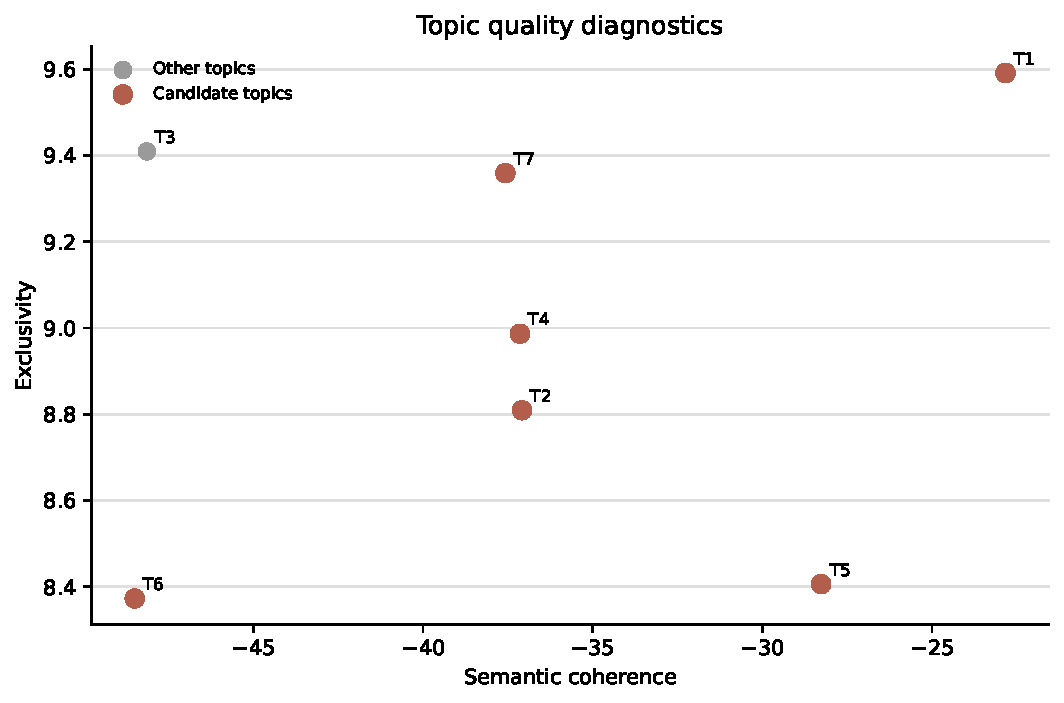
\includegraphics[width=0.78\textwidth]{figure5_topic_quality.pdf}
\caption{Topic-quality diagnostics (semantic coherence vs.\ exclusivity).
Candidate masculine formations in colour; the Gothic-romance control in grey.}
\label{fig:quality}
\end{figure}

\subsection{Which formations separate, and when}
A second, more revealing result concerns not the seven-topic solution alone but
the order in which the formations emerge as the model grows
(Table~\ref{tab:coverage}, Fig.~\ref{fig:modelcomp}). Four families---domestic paternalism, gentlemanly
status, imperial adventure, sentimental manhood---separate by $K=5$; aristocratic
chivalry separates at $K=6$; professional breadwinning at $K=7$; and Christian
moralism not until $K=9$. Even then it does not form a tidy devotional topic: at
$K=9$ the religious vocabulary (\emph{religion}, \emph{christian}, \emph{divine})
emerges blended with philosophical and national-historical language
(\emph{philosopher}, \emph{nation}, \emph{government}, with exemplars such as
\emph{Hypatia} and \emph{Romola}), and its appearance fragments the domestic
topic. We read this not as the absence of religious masculinity but as evidence
of \emph{dispersion}: religious vocabulary is spread across domestic-household
and historical-intellectual registers rather than concentrated, so at $K=7$ it
has no distinct topic of its own. In this corpus, moral-religious manhood is
articulated through other formations rather than as a freestanding one---a
pattern consistent with accounts of Victorian domestic and moral manliness
\citep{tosh1999mans,sussman1995victorian}. All seven families are retained as the
theoretical lens; their differential separability is itself a finding about the
corpus, not a defect of the model.

\begin{table}[htbp]
\centering
\caption{Family coverage across $K$. All seven theory-driven families are
retained as the interpretive lens; the column gives the smallest $K$ at which
each separates as a distinct topic. The Gothic-romance topic is a non-masculine
control and is not a family.}
\label{tab:coverage}
\small
\begin{tabular}{l l c c}
\toprule
Family & Example keywords & First $K$ recovered & Status at $K=7$ \\
\midrule
Domestic Paternalism     & child, family, father, mother    & 5 & Separate \\
Gentlemanly Status       & conduct, dignity, gentleman, sir & 5 & Separate \\
Imperial Adventure       & army, captain, sea, ship         & 5 & Separate \\
Sentimental Manhood      & affection, feeling, grief, love  & 5 & Separate \\
Aristocratic Chivalry    & castle, chivalry, knight, prince & 6 & Separate \\
Professional Breadwinner & bank, business, money, trade     & 7 & Separate \\
Christian Moralism       & christian, church, faith, soul   & 9 & Fused with Domestic \\
\bottomrule
\end{tabular}
\end{table}

\begin{figure}[htbp]
\centering
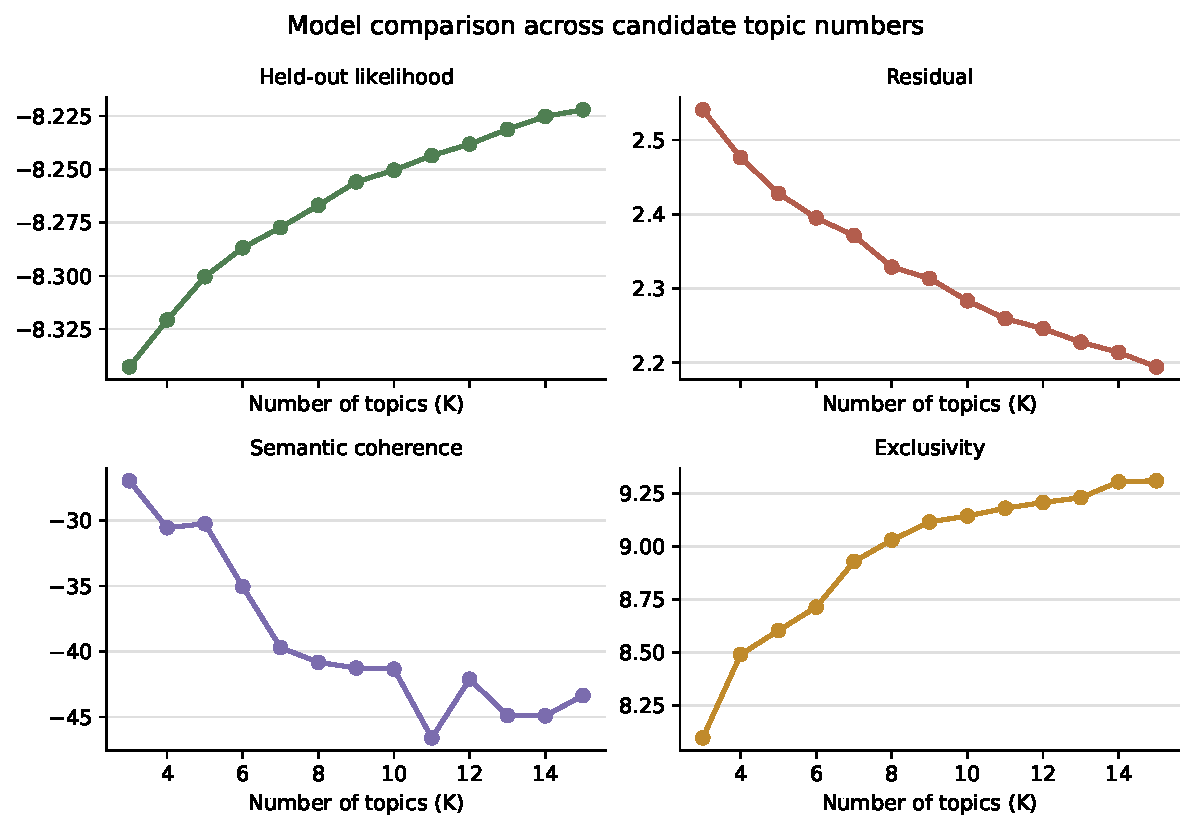
\includegraphics[width=0.9\textwidth]{figure2_model_comparison.pdf}
\caption{Model comparison for $K=3$--$15$. Held-out likelihood, residuals, and
exclusivity improve monotonically with $K$, while semantic coherence peaks at low
$K$ and declines. The choice of $K=7$ rests on the substantive criterion in
Section~\ref{sec:modelsel}, not on these curves alone.}
\label{fig:modelcomp}
\end{figure}

\subsection{Historical trajectories (RQ2)}
Figure~\ref{fig:trajectories} shows novel-level prevalence by period with 95\%
bootstrap intervals; Figure~\ref{fig:heatmap} gives the same values as a heatmap.
Every between-period change (Early Modernist minus Georgian) is statistically
robust under the difference bootstrap, but the changes differ enormously in
size. Two signals dominate: professional breadwinning rises by
$+0.351$ $[+0.264, +0.441]$ ($p<0.001$; from $0.021$ to $0.372$), and sentimental
manhood falls by $-0.332$ $[-0.399, -0.266]$ ($p<0.001$; from $0.352$ to
$0.020$). Domestic paternalism rises ($+0.147$ $[+0.096, +0.202]$, $p<0.001$;
peaking in the Early and Late Victorian periods at $0.244$ and $0.249$) and
imperial adventure climbs to a Late Victorian plateau ($+0.150$
$[+0.071, +0.229]$, $p<0.001$). The Gothic control falls steeply
($0.188 \rightarrow 0.036$), confirming that the model tracks broad
literary-historical structure rather than gendered vocabulary alone.

The two ``rank'' formations also decline significantly, but modestly. Gentlemanly
status falls by $-0.074$ $[-0.136, -0.016]$ ($p=0.014$; from a $0.198$ Early
Victorian peak to $0.077$) and aristocratic chivalry by $-0.090$
$[-0.154, -0.026]$ ($p=0.004$). The ``rank-to-work'' narrative is therefore
asymmetric not in \emph{significance} but in \emph{magnitude}: the rise of
professional-commercial masculinity is roughly five times larger than the
erosion of gentlemanly recognition. A reading on which gentility is simply
swapped for work overstates the second half of the exchange; the data show a
large new formation emerging \emph{alongside} a real but modest decline of the
old. (Inspecting per-group interval overlap, by contrast, would have wrongly
labeled the gentlemanly decline ``non-significant''---an artifact of that
heuristic, not of the data.)

\begin{figure}[htbp]
\centering
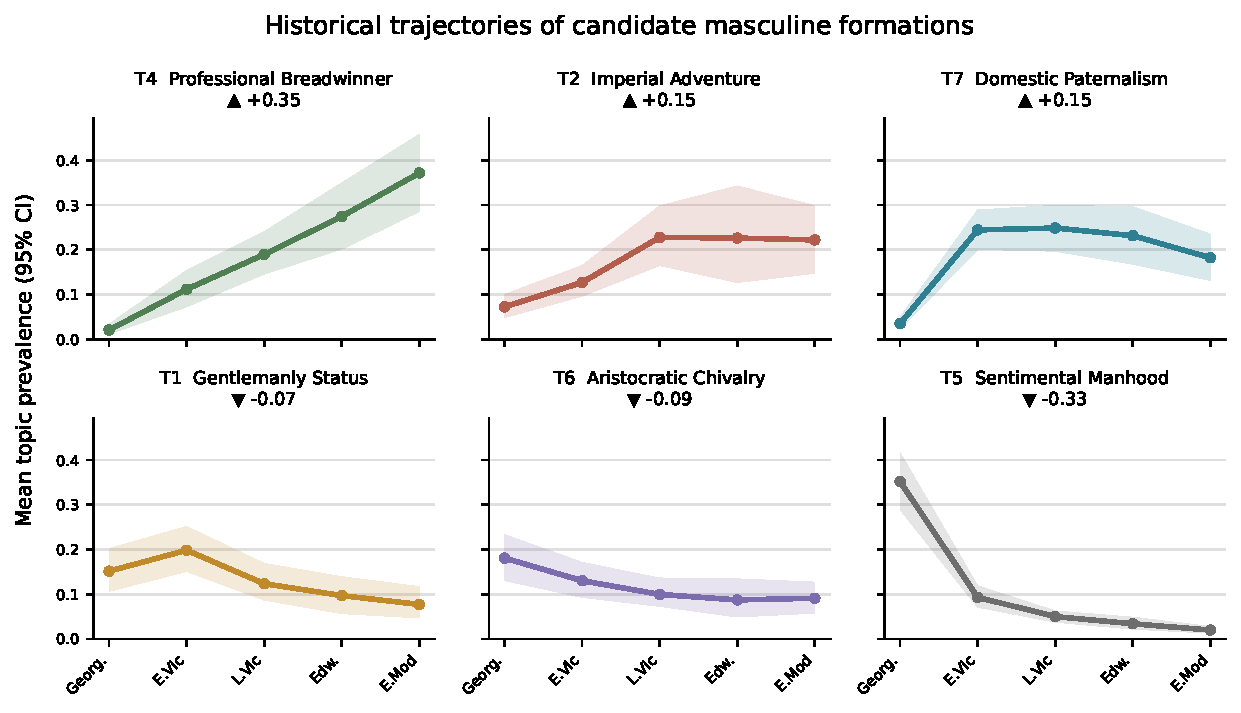
\includegraphics[width=\textwidth]{figure1_period_small_multiples.pdf}
\caption{Historical trajectories of the six candidate masculine formations
(novel-level mean prevalence with 95\% bootstrap intervals), ordered by net
change. Rising: professional breadwinning, imperial adventure, domestic
paternalism. Declining: gentlemanly status, aristocratic chivalry, sentimental
manhood.}
\label{fig:trajectories}
\end{figure}

\begin{figure}[htbp]
\centering
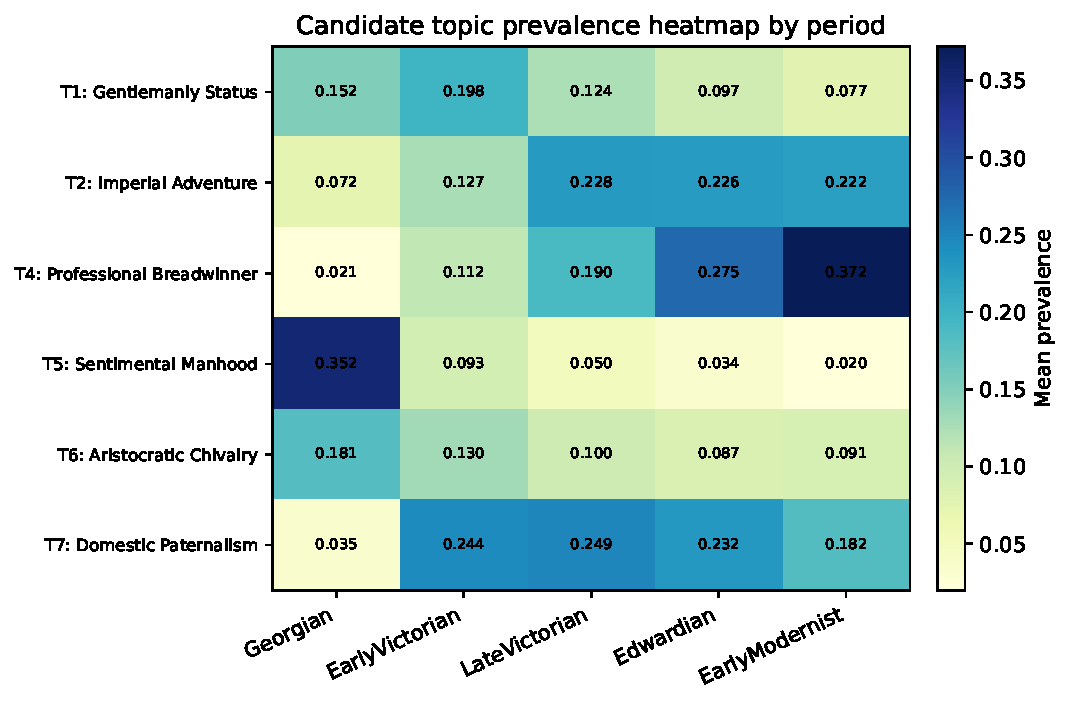
\includegraphics[width=0.88\textwidth]{figure4_candidate_topic_period_heatmap.pdf}
\caption{Heatmap of novel-level mean prevalence by period for the six candidate
formations.}
\label{fig:heatmap}
\end{figure}

\subsection{Author gender (RQ3)}
Figure~\ref{fig:gender} and Table~\ref{tab:gender} report novel-level prevalence
by author gender. Under the difference bootstrap, all six male--female contrasts
are statistically robust: female authors are higher on gentlemanly status
($-0.087$ male$-$female, $p<0.001$), domestic paternalism ($-0.089$, $p<0.001$),
and sentimental manhood ($-0.100$, $p=0.001$), whereas male authors are higher on
imperial adventure ($+0.103$, $p<0.001$), aristocratic chivalry ($+0.107$,
$p<0.001$, the largest gap), and professional breadwinning ($+0.074$,
$p=0.005$). The professional-breadwinning gap is worth a note: the per-group
intervals in Fig.~\ref{fig:gender} nearly touch, yet the paired difference is
robust---another instance in which interval overlap understates a real
difference. Because author gender enters only as a secondary covariate, we make
no causal claim about gendered authorship; the contrasts describe association,
not authorial intent.

\begin{figure}[htbp]
\centering
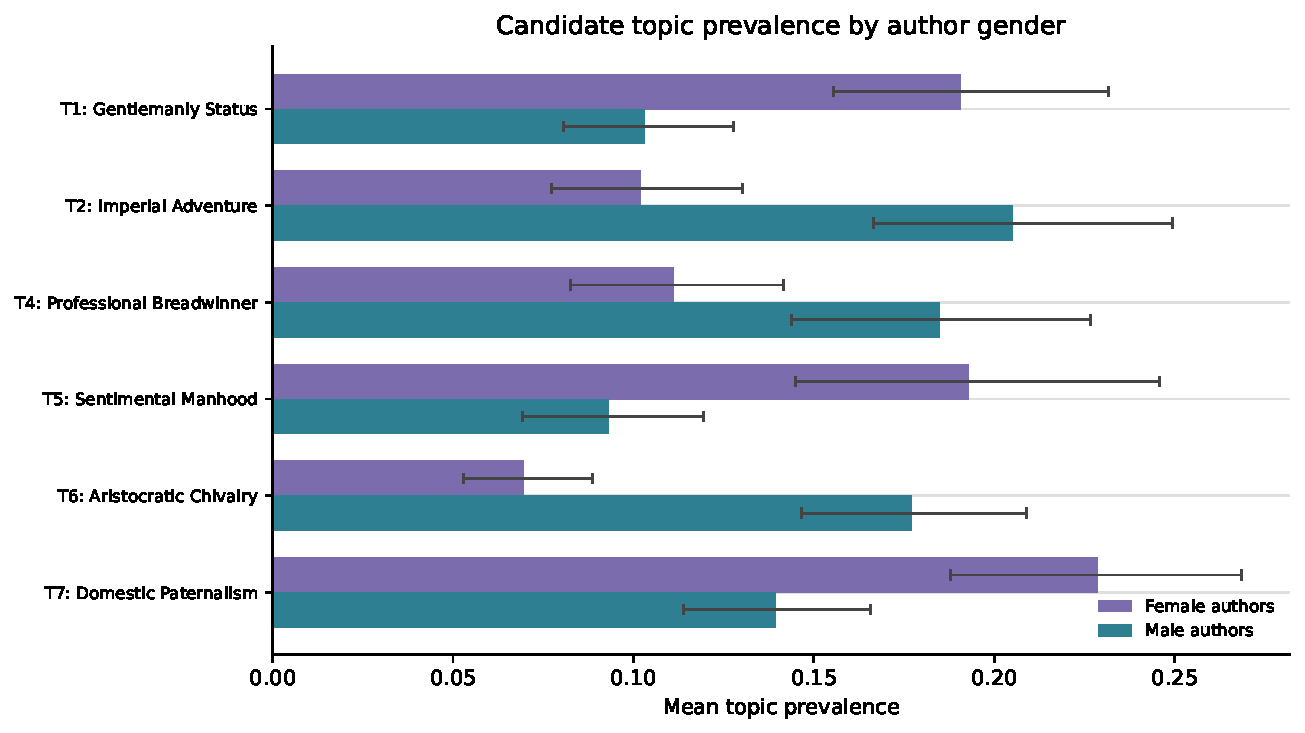
\includegraphics[width=0.95\textwidth]{figure3_author_gender_candidate_topics.pdf}
\caption{Novel-level mean prevalence by author gender with 95\% bootstrap error
bars (per-group). All six male--female differences are robust under the
difference bootstrap (Table~\ref{tab:gender}); for professional breadwinning the
per-group bars nearly overlap even though the paired difference is significant
($p=0.005$).}
\label{fig:gender}
\end{figure}

\begin{table}[htbp]
\centering
\caption{Novel-level mean prevalence by author gender, with the bootstrapped
male$-$female difference and its two-sided $p$-value (candidate formations). All
six contrasts are statistically robust.}
\label{tab:gender}
\small
\begin{tabular}{l c c c c}
\toprule
Formation & Female & Male & M$-$F diff [95\% CI] & $p$ \\
\midrule
Gentlemanly Status       & 0.191 & 0.103 & $-0.087$ $[-0.132, -0.043]$ & $<0.001$ \\
Domestic Paternalism     & 0.229 & 0.139 & $-0.089$ $[-0.139, -0.042]$ & $<0.001$ \\
Sentimental Manhood      & 0.193 & 0.093 & $-0.100$ $[-0.158, -0.042]$ & $0.001$ \\
Imperial Adventure       & 0.102 & 0.205 & $+0.103$ $[+0.054, +0.153]$ & $<0.001$ \\
Aristocratic Chivalry    & 0.070 & 0.177 & $+0.107$ $[+0.070, +0.143]$ & $<0.001$ \\
Professional Breadwinner & 0.111 & 0.185 & $+0.074$ $[+0.023, +0.125]$ & $0.005$ \\
\bottomrule
\end{tabular}
\end{table}

\section{Discussion}

The substantive result is a reweighting, not a replacement. Across the corpus,
fiction shifts from masculine formations organized around gentility, rank, and
sentiment toward one organized around work, money, and the city, while the older
formations persist at lower prevalence rather than disappearing. This is a
stronger claim than a word-frequency trend, because it rests on topics---stable
constellations of co-occurring words---yet a weaker claim than an account of
masculine character, because the method models lexical environments rather than
narrative agency.

Three features of the results deserve emphasis. First, the trajectories show
\emph{convergent validity} with independent historiography: domestic paternalism
peaks in the high-Victorian decades \citep{tosh1999mans}, imperial adventure
crests in the late century, and the professional-commercial formation rises into
modernity as status is reorganized from inherited rank toward labor and capital.
That an unsupervised model recovers a periodization scholars established by close
reading \emph{corroborates} the formations; it does not prove them, since the
labels remain interpretive and period effects may partly reflect genre and corpus
composition (for instance, the late-century concentration of adventure and urban
fiction). Second, the model supplies a mild corrective: although the ``decline of
the gentleman'' is statistically robust, it is roughly five times smaller in
magnitude than the rise of the breadwinner, so the common framing of a symmetric
swap from gentility to work overstates the losing side of the ledger. This
asymmetry of magnitude is easy to miss without an explicit difference test, and
is a concrete payoff of resampling whole novels and testing the contrast directly
rather than reading significance off overlapping per-group intervals.

Third, and most general, the study clarifies what topic modeling can and cannot
establish about plurality. It can show that multiple masculine formations are
lexically distinguishable and that their prevalence is reweighted over time---
operationalizing Connell's plurality at corpus scale. It cannot certify
\emph{how many} formations exist: the number of topics $K$ is a researcher choice,
the diagnostics conflict on the ``best'' $K$ (Section~\ref{sec:modelsel}), and the
families separate at different $K$ rather than all at once. The late emergence of
a standalone Christian-moralism topic is, on this reading, evidence of
fusion---religious manhood expressed through domesticity---rather than evidence
that the formation is absent. Treating the count of masculinities as an empirical
output would reintroduce exactly the circularity we set out to avoid.

\section{Limitations}

Four limitations bound these claims. First, the study includes no independent
human annotation, so it can say that topics are meaningfully \emph{associated}
with recognized masculine roles, not that they \emph{are} masculinity. Second,
with 150 novels, period effects may partly reflect genre distribution, author
selection, and availability biases, and the smaller late-period samples produce
wider intervals. Third, although novel-level aggregation addresses the dependence
among same-novel segments, a fully hierarchical model would be preferable.
Fourth, some topics remain contaminated by character names (e.g.\ \emph{tom},
\emph{emily}, \emph{margaret}) despite the document-specificity filter, and
several labels (notably imperial adventure and sentimental manhood) are broader
than their names; both are reasons to read the formations as maps rather than as
definitions.

\section{Conclusion}

Using structural topic modeling, this article maps how masculine social
formations are reweighted across English fiction from 1771 to 1930. Six of seven
theory-driven formations separate as distinct topics; the seventh, Christian
moralism, remains fused with domesticity until a larger model size. Novel-level
bootstrap intervals show a robust rise of professional-commercial masculinity and
a robust decline of a sentimental register, alongside a markedly weaker decline of
gentlemanly recognition. Beyond this case, the study offers a disciplined
template for applying topic models to theoretical constructs: treat the
categories as a lens rather than a target, fix model size on a substantive
criterion, quantify uncertainty at the level of genuinely independent
observations, and validate against external scholarship. On that basis, computational analysis can make the
plurality and historical movement of masculine formations measurable---while
leaving the question of their number where it belongs, with theory and
interpretation rather than with the model.

\section*{Data and code availability}
The custom code central to this study---segmentation, STM preparation, model
estimation, reporting, model comparison, family-coverage analysis, and
figure generation (\texttt{proposal2\_segment.py}, \texttt{proposal2\_stm\_prep.py},
\texttt{proposal2\_run\_stm.R}, \texttt{proposal2\_stm\_report.py},
\texttt{proposal2\_family\_coverage.py}, \texttt{proposal2\_hssc\_figures.py})---
together with the derived segment metadata, STM input matrices, topic-word
tables, model-comparison outputs, bootstrap summaries, and figure scripts, are
available in an anonymized repository for review at [URL] and will be deposited
in a persistent, DOI-providing archive (OSF/Zenodo/figshare) on acceptance. The
underlying corpus is openly available as Andrew Piper's txtLAB Novel450 dataset
\citep{piper2016txtlab}.

\section*{Ethics declarations}
Ethical approval was not required: the study analyses published literary texts
and involves no human participants or personal data. The authors declare no
competing interests.

\appendix
\section{Theory-driven family keyword lists}
\label{app:families}
The seven masculine families are an a-priori interpretive lens (Section~4.3). A
topic is flagged as a candidate for a family when at least two of its
highest-probability or FREX words fall in that family's list. The lists below are
the exact vocabularies used; they are applied only \emph{after} estimation and
never enter model fitting or the choice of $K$. The Gothic-romance topic matches
no family and is treated as a non-masculine contextual control.

\smallskip
\noindent\textbf{Gentlemanly Status:} address, character, conduct, courtesy,
dignity, gentleman, gentlemen, honor, honour, lady, ladyship, polite, propriety,
rank, reputation, respect, respectable, sir, society.

\noindent\textbf{Domestic Paternalism:} boy, care, child, children, daughter,
family, father, girl, home, household, husband, marriage, married, mother, parent,
son, wife.

\noindent\textbf{Aristocratic Chivalry:} baron, castle, chivalry, court, crown,
duke, hero, highness, honor, honour, horse, king, knight, lord, master, noble,
prince, queen, royal, sword.

\noindent\textbf{Professional Breadwinner:} bank, business, capital, clerk,
credit, debt, dollar, employment, fortune, income, labor, labour, merchant, money,
office, pound, profession, property, trade, work.

\noindent\textbf{Imperial Adventure:} army, battle, camp, captain, colonial,
colony, courage, danger, empire, endurance, enemy, fight, forest, frontier,
indian, island, jungle, native, officer, rifle, scout, sea, ship, soldier, travel,
voyage, war, wilderness.

\noindent\textbf{Christian Moralism:} christian, church, conscience, duty, evil,
faith, god, goodness, heaven, holy, minister, moral, piety, prayer, priest,
religion, sin, soul, truth, virtue.

\noindent\textbf{Sentimental Manhood:} affection, beloved, dear, emotion, feeling,
grief, happiness, joy, love, melancholy, misery, passion, sensibility, sentiment,
sorrow, sympathy, tender.

\bibliographystyle{plainnat}
\bibliography{references}

\end{document}
